\documentclass[12pt,utf8,notheorems,compress]{beamer}
\usepackage{etex}

\usepackage[english]{babel}

\usepackage{amsmath,amssymb,tabto}

\usepackage[protrusion=true,expansion=false]{microtype}

\setlength\parskip{\medskipamount}
\setlength\parindent{0pt}

\newcommand{\RR}{\mathbb{R}}
\newcommand{\Set}{\mathrm{Set}}

\title{Markov chains and MCMC methods}
\author[Kleine Bayessche AG]{%
  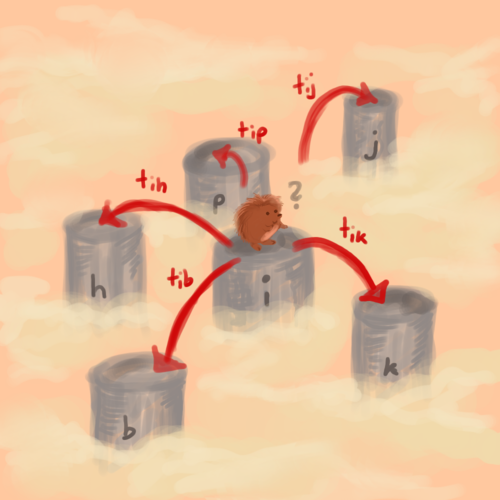
\includegraphics[scale=0.3]{markov.png}
  }
\date{7. November 2014}

%\usetheme{Warsaw}  %Warsaw, Berkeley?
\usetheme{Warsaw}
\useoutertheme[subsection=false]{miniframes}
\usecolortheme{seahorse}
\usefonttheme{serif}
\usepackage{kurier}
\useinnertheme{rectangles}
%\usepackage{bookman}
%\setbeamercovered{transparent}

\setbeamertemplate{frametitle}[default][colsep=-4bp,rounded=false,shadow=false,center]

\setbeamertemplate{navigation symbols}{}
%\setbeamertemplate{footline}{}
%\setbeamertemplate{headline}{}

%\beamertemplateboldcenterframetitle
%\setbeamerfont{frametitle}{size={\Large}}

\newcommand*\oldmacro{}%
\let\oldmacro\insertshorttitle%
\renewcommand*\insertshorttitle{%
  \oldmacro\hfill\insertframenumber\,/\,\inserttotalframenumber\hfill}

\newenvironment{changemargin}[2]{%
  \begin{list}{}{%
    \setlength{\topsep}{0pt}%
    \setlength{\leftmargin}{#1}%
    \setlength{\rightmargin}{#2}%
    \setlength{\listparindent}{\parindent}%
    \setlength{\itemindent}{\parindent}%
    \setlength{\parsep}{\parskip}%
  }%
  \item[]}{\end{list}}

\newcommand{\hil}[1]{{\usebeamercolor[fg]{item}{#1}}}

\begin{document}

\setbeameroption{show notes}
\setbeamertemplate{note page}[plain]

\frame{\titlepage}
%\frame[t]{\frametitle{Gliederung}\begin{minipage}{\textwidth}\begin{small}\tableofcontents\end{small}\end{minipage}}
\frame[t]{\frametitle{Outline}\tableofcontents}

\section[Basics]{Basics on Markov chains}

\frame[t]{\frametitle{What is a Markov chain?}
  \begin{itemize}
    \item A Markov chain is a system which undergoes transitions from one state
    to another according to probabilities~$P(X' = j \,|\, X = i) =: T_{ij}$.
    \vfill
    \item More abstractly, a Markov chain on a state space~$S$ is a map~$S \to
    D(S)$, where~$D(S)$ is the set of probability measures on~$S$.
    \vfill
    \item Categorically, a Markov chain is a coalgebra for the functor~$D :
    \Set \to \Set$.
  \end{itemize}
}

\note{
  The following systems can be modeled by Markov chains:
  \begin{itemize}
  \item the peg in the game of snakes and ladders
  \item a random walk
  \item the weather, if we oversimplify a lot
  \item randomly surfing on the web
  \end{itemize}

  The following cannot:

  \begin{itemize}
  \item the state of a game of blackjack
  \end{itemize}
}

\frame[t]{\frametitle{Basic theory on Markov chains}
  \begin{itemize}
    \item The transition matrix is a \hil{stochastic matrix}:
    \[ T_{ij} \geq 1, \qquad \textstyle\sum\limits_j T_{ij} = 1. \]
    \item If~$p \in \RR^S$ is a distribution of the initial state, \\
    then $p^\mathrm{T} \cdot T^N \in \RR^S$ is the distribution of the~$N$'th
    state.
    \item If the Markov chain is \hil{irreducible} and \hil{aperiodic},
    $p^\mathrm{T} \cdot T^N$ approaches a unique \hil{limiting
    distribution~$p^\infty$}
    independent of~$p$ as~$N \to \infty$.
    \item A sufficient condition for~$p^\infty = q$ is the \hil{detailled balance
    condition}
    \[ q_i T_{ij} = q_j T_{ji}. \]
  \end{itemize}
}


\section[Chat bot]{Live demo: an IRC chat bot}
\frame{
  \begin{center}
    \huge
    Live demo: an IRC chat bot
  \end{center}
}


\section[Sampling]{Sampling from distributions}
\frame[t]{\frametitle{How can we sample from distributions?}
  Given a density~$f$, want independent samples~$x_1,x_2,\ldots$
  \bigskip

  \only<1-2>{\begin{itemize}
  \item If the inverse of the cumulative distribution function~$F$ is available:
  \bigskip

        \begin{enumerate}
        \item Sample~$u \sim U(0,1)$. \\[0.5em]
        \item Output~$x := F^{-1}(u)$.
        \end{enumerate}

  \bigskip
  \item<2> Unfortunately, calculating~$F^{-1}$ is expensive in general.
  \end{itemize}}

  \only<3-4>{\begin{itemize}
  \item If some other sampleable density~$g$ with $f \leq M g$ is
  available, where~$M \geq 1$ is a constant, we can use \hil{rejection sampling}:
  \bigskip

  \begin{enumerate}
  \item Sample~$x \sim g$. \\[0.5em]
  \item Sample~$u \sim U(0,1)$. \\[0.5em]
  \item If~$u < \frac{1}{M} f(x)/g(x)$, output~$x$; else, retry.
  \end{enumerate}

  \bigskip
  \item<4> Works even if~$f$ is only known up to a constant factor.
  \item<4> Acceptance probability is~$1/M$, this might be small.
  \end{itemize}}
}

\note{
  \fontsize{8pt}{9.6}\selectfont
  \begin{itemize}
    \item Proof that the easy sampling algorithm is correct:
          \[ P(F^{-1}(U) \leq x) = P(U \leq F(x)) = F(x). \]

    \item Acceptance probability in rejection sampling:
          \begin{align*}
            P(U < \tfrac{1}{M} f(G)/g(G)) &=
             E(\tfrac{1}{M} f(G)/g(G)) \\&=
             \tfrac{1}{M} \cdot \int f(x)/g(x) \cdot g(x) \,dx =
             \tfrac{1}{M}.
          \end{align*}
    \item Proof of correctness of rejection sampling:
          \begin{align*}
            P(G \leq x \,\wedge\, U < \tfrac{1}{M} f(G)/g(G))
            &= \int P(G \leq x \,\wedge\, U < \tfrac{1}{M} f(G)/g(G) \ |\ G = t) g(t)\,dt \\
            &= \int \boldsymbol{1}_{t \leq x} \cdot P(U < \tfrac{1}{M} f(t)/g(t)) \cdot g(t) \,dt \\
            &= \int \boldsymbol{1}_{t \leq x} \cdot \tfrac{1}{M} f(t)/g(t) \cdot g(t) \,dt \\
            &= \tfrac{1}{M} F(x), \\[1em]
            \text{so}\quad P(G \leq x \ |\ U < \tfrac{1}{M} f(G)/g(G)) &= F(x).
          \end{align*}
  \end{itemize}
}

\frame[t]{\frametitle{Markov chain Monte Carlo methods}
  Given a density~$f$, want independent samples~$x_1,x_2,\ldots$

  \begin{enumerate}
    \item Construct a Markov chain with limiting density~$f$.
    \item Draw samples from the chain.
    \item Discard first samples (burn-in period).
    \item From the remaining samples, retain only every~$N$'th.
  \end{enumerate}

  Works very well in practice.
}

\frame[t]{\frametitle{Metropolis--Hastings algorithm}
  Given a density~$f$, want independent samples~$x_1,x_2,\ldots$

  Let~$g(y,x)$ be such that for any~$x$, $g(\cdot,x)$ is sampleable.
  Set~$B(x,y) := \frac{f(y) g(x,y)}{f(x) g(y,x)}$.

  \begin{enumerate}
    \item Initialize~$x$. \\[0.5em]
    \item Sample~$u \sim U(0,1)$. \\[0.5em]
    \item Sample~$y \sim g(\cdot,x)$. \\[0.5em]
    \item If~$u < B(x,y)$, set~$x := y$; else, keep~$x$ unchanged. \\[0.5em]
    \item Output~$x$ and go back to step~2.
  \end{enumerate}

  Works even if~$f$ and~$g$ are only known up to constant factors.
}

\note{
  \begin{itemize}
    \item The Metropolis algorithm was first published in an 1953 paper \emph{Equation of
    State Calculations by Fast Computing Machines} by Metropolis, Rosenbluth,
    Augusta Teller, and Edward Teller. Hastings' addition was in 1970.

    \item Special case: $g(x,y) = g(y,x)$, then~$B(x,y) = f(y)/f(x)$; this is
    the original Metropolis algorithm.

    \item Example: $g(\cdot,x) = N(x,\sigma^2)$.

    \item Set~$A(x,y) := \min\{1,\,B(x,y)\}$.

    \item Transition matrix (really, kernel):
    \[ T(x,y) = \hat g(y,x) A(x,y) + \delta(x,y) \int (1-A(x,z)) \hat g(z,x) \,dz. \]

    \item Balance condition (for~$x \neq y$):
    \[ f(x) T(x,y) = \min\{ f(x) \hat g(y,x),\, f(y) \hat g(x,y) \} =
      f(y) T(y,x). \]
  \end{itemize}
}


\section[Integrals]{Evaluating integrals over high-dimensional domains}
\frame[t]{\frametitle{Evaluating integrals}
  How can we evaluate integrals
  \[ \int a(x) \, f(x) \,dx, \]
  where~$f$ is a density on a high-dimensional domain?

  \begin{itemize}
    \item $\int_a^b$: \tabto{1.045cm}standard numerical quadrature
    \item $\int_{-\infty}^\infty$: \tabto{1.045cm}numerical quadrature after coordinate
    transform
    \item $\int_{\RR^n}$: \tabto{1.045cm}iterated numerical quadrature
  \end{itemize}

  \pause
  These techniques sample the domain uniformly and require many
  evaluations of the integrand.
}

\note{
  \begin{itemize}
    \item Evaluation of such integrals is, of course, important in Bayesian
    learning and elsewhere.
    \item Note that adaptive numerical quadrature rules do exist.
  \end{itemize}
}

\frame[t]{\frametitle{The Monte Carlo approach}
  Draw indep.\@ samples~$x_1,\ldots,x_N$ from~$f$ and approximate
  \[ f \approx \frac{1}{N} \sum_{i=1}^N \delta_{x_i}, \qquad
  I := \int a(x) \, f(x) \,dx \approx
    \frac{1}{N} \sum_{i=1}^N f(x_i) =: I_N. \]

  \begin{itemize}
    \item $E(I_N) = I$. \\[0.5em]
    \item $\operatorname{Var}(I_N) = \operatorname{Var}_f(a) / N$.
    \item $I_N \longrightarrow I$ almost surely (strong law of large numbers). \\[0.5em]
  \end{itemize}
  \bigskip

  To sample~$f$, use Markov chain techniques; obtain \hil{MCMC methods}.
  These made Bayesian ideas useful in practice.
}


%\section{Further study}
%\frame[t]{\frametitle{Further study}
%  \begin{itemize}
%    \item Survey the extensive literature on Markov chains.
%    \item Write a semantically driven chat bot.
%    \item In the view of quantum mechanics as a generalization of probability
%    theory, what is the meaning of MCMC algorithms?
%  \end{itemize}
%}

\end{document}

http://jtobin.ca/flat-mcmc/
